\section{Confronto tra PBWT e RLPBWT}
Al fine di analizzare i risultati ottenuti si sono confrontate 5 varianti della
\textit{RLPBWT}:
\begin{itemize}
  \item \textit{RLPBWT na\"{i}ve}
  \item \textit{RLPBWT con bitvector}
  \item \textit{RLPBWT con pannello completo e threshold}
  \item \textit{RLPBWT con pannello compresso (SLP) e threshold}
  \item \textit{RLPBWT con pannello compresso (SLP) e LCE query}  
\end{itemize}
Confrontandole con l'implementazione originale dell'algoritmo 5 di Durbin,
nominato \textit{MatchIndexed}. Studiando la repository di Durbin inoltre si è
scoperto l'esistenza di un ulteriore algoritmo, non descritto
formalmente nel paper del 2014 \cite{pbwt} ma solo citato in una tabella, che
considera in un unico panello sia il pannello che l'insieme delle query ed
effettua il matching interno al pannello stesso, calcolando in modo dinamico
l'indicizzazione ad ogni colonna. Nonostante l'algoritmo presenti limiti dal
punto di vista dell'estendibilità ad altre problematiche, avendo che le varianti
della \textit{PBWT} citate in sezione \ref{secpbwt} si basano, nel caso di
\textit{SMEM} 
con aplotipi esterni, sulle idee dell'algoritmo 5, esso risulta essere davvero
molto performante sia dal punto di vista del tempo macchina che della memoria
occupata. A causa di ciò, per completezza, tale algoritmo, chiamato
\textit{MatchDynamic}, è stato incluso nei risultati sperimentali, pur
mancandone una trattazione teorica approfondita.
\subsection{Analisi spaziale}
Lo scopo principale di questa tesi era la riduzione delle informazioni in
memoria necessarie a permette il mapping, quindi in primis si sono valutati i
vari risultati dal punto di vista della memoria.
\subsubsection{Dimensioni dell'SLP}
Prima ancora di affrontare i requisiti
in memoria dell'intera struttura è interessante analizzare le capacità di
compressione che si ha con l'uso degli \textit{SLP}, grazie ai due tool sopra
citati. In figura \ref{fig:slpres1} si può iniziare ad apprezzare l'efficacia di
tale grammatica. Si nota infatti come, per quanto i pannelli siano di dimensione
modesta, hanno un peso che varia in un range di un centinaio di megabytes mentre
gli \textit{SLP} relativi nel centinaio di kilobytes. Si ha infatti:
\begin{table}[H]
  \centering
  \begin{tabular}{c|c|c|c|c}
    \textbf{altezza} & \textbf{larghezza} & \textbf{SLP (\textit{kb})}
    & \textbf{MACs (\textit{kb})} & \textbf{\%}\\
    \hline
    20000 & 4294 & 228.13 & 84050.48 & 0.2714\\
    21000 & 4294 & 238.83 & 88243.83 & 0.2707\\
    22000 & 4294 & 243.04 & 92437.18 & 0.2629\\
    23000 & 4294 & 250.37 & 96630.53 & 0.2591\\
    24000 & 4294 & 272.72 & 100823.87 & 0.2705\\
    25000 & 4294 & 278.22 & 105017.22 & 0.2649\\
    26000 & 4294 & 283.57 & 109210.57 & 0.2597\\
    27000 & 4294 & 288.62 & 113403.92 & 0.2545\\
    28000 & 4294 & 293.85 & 117597.27 & 0.2499\\
    29000 & 4294 & 298.76 & 121790.62 & 0.2453\\
  \end{tabular}
\end{table}
Notando come, per pannelli di grandezza simile, pare si abbia una compressione
proporzionale alla dimensione del pannello.\\
\begin{figure}
  \centering
  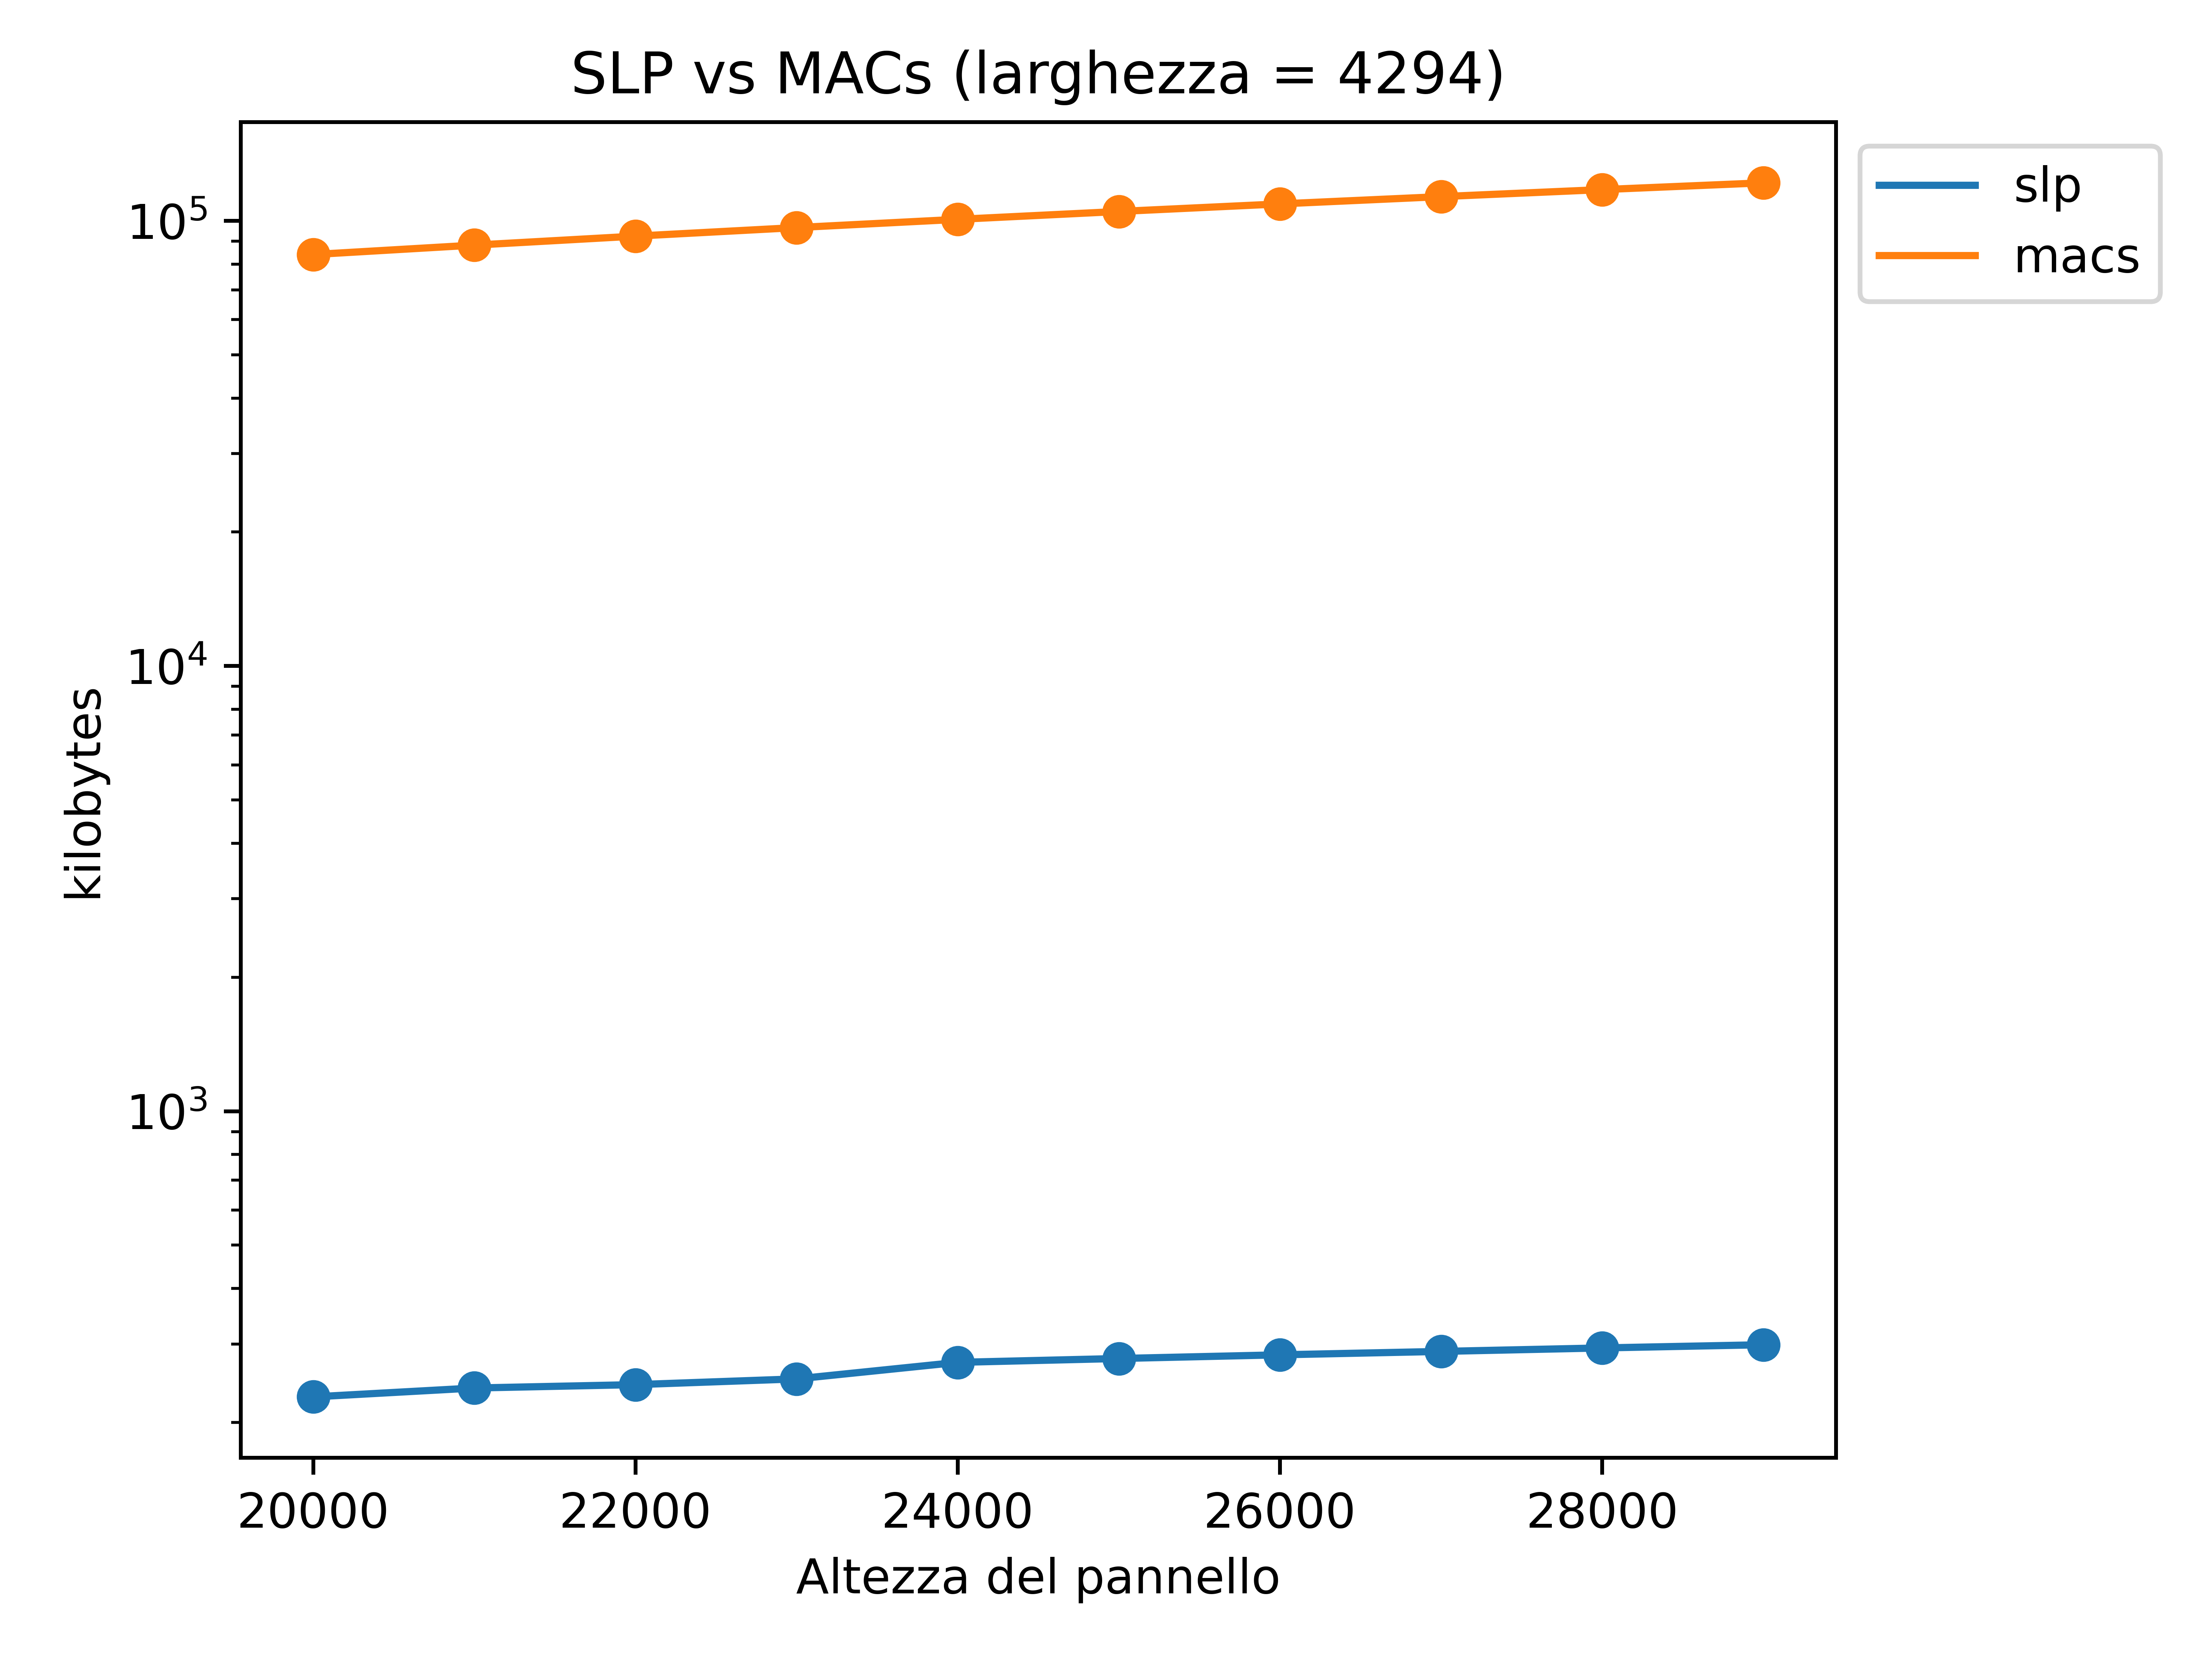
\includegraphics[scale = 0.6]{img/slp_vs_macs.png}
  \caption{Confronto delle dimensioni, espresse in kilobytes, dei pannelli in
    formato \texttt{macs} e dei rispettivi \textit{SLP}. Il grafico è in scala
    logaritmica.}
  \label{fig:slpres1}
\end{figure}
Andando a vedere pannelli molto più grossi si nota come il rateo di
compressione continui essere proporzionale alla dimensione del pannello e,
nonostante il esso cresca di 
dimensione, la grandezza dell'\textit{SLP} resta molto piccola:
\begin{table}[H]
  \centering
  \begin{tabular}{c|c|c|c|c}
    \textbf{altezza} & \textbf{larghezza} & \textbf{SLP (\textit{kb})}
    & \textbf{MACs (\textit{kb})} & \textbf{\%}\\
    \hline
    100000 & 358653 & 14771.0 & 35042963.54 & 0.0422\\
    100000 & 100000 & 9077.88 & 9075120.49 & 0.1\\
    100000 & 46538 & 8017.09 & 4448994.19 & 0.1802\\
  \end{tabular}
\end{table}
Tale risultato è anche apprezzabile in figura \ref{fig:slpres2}.
\begin{figure}
  \centering
  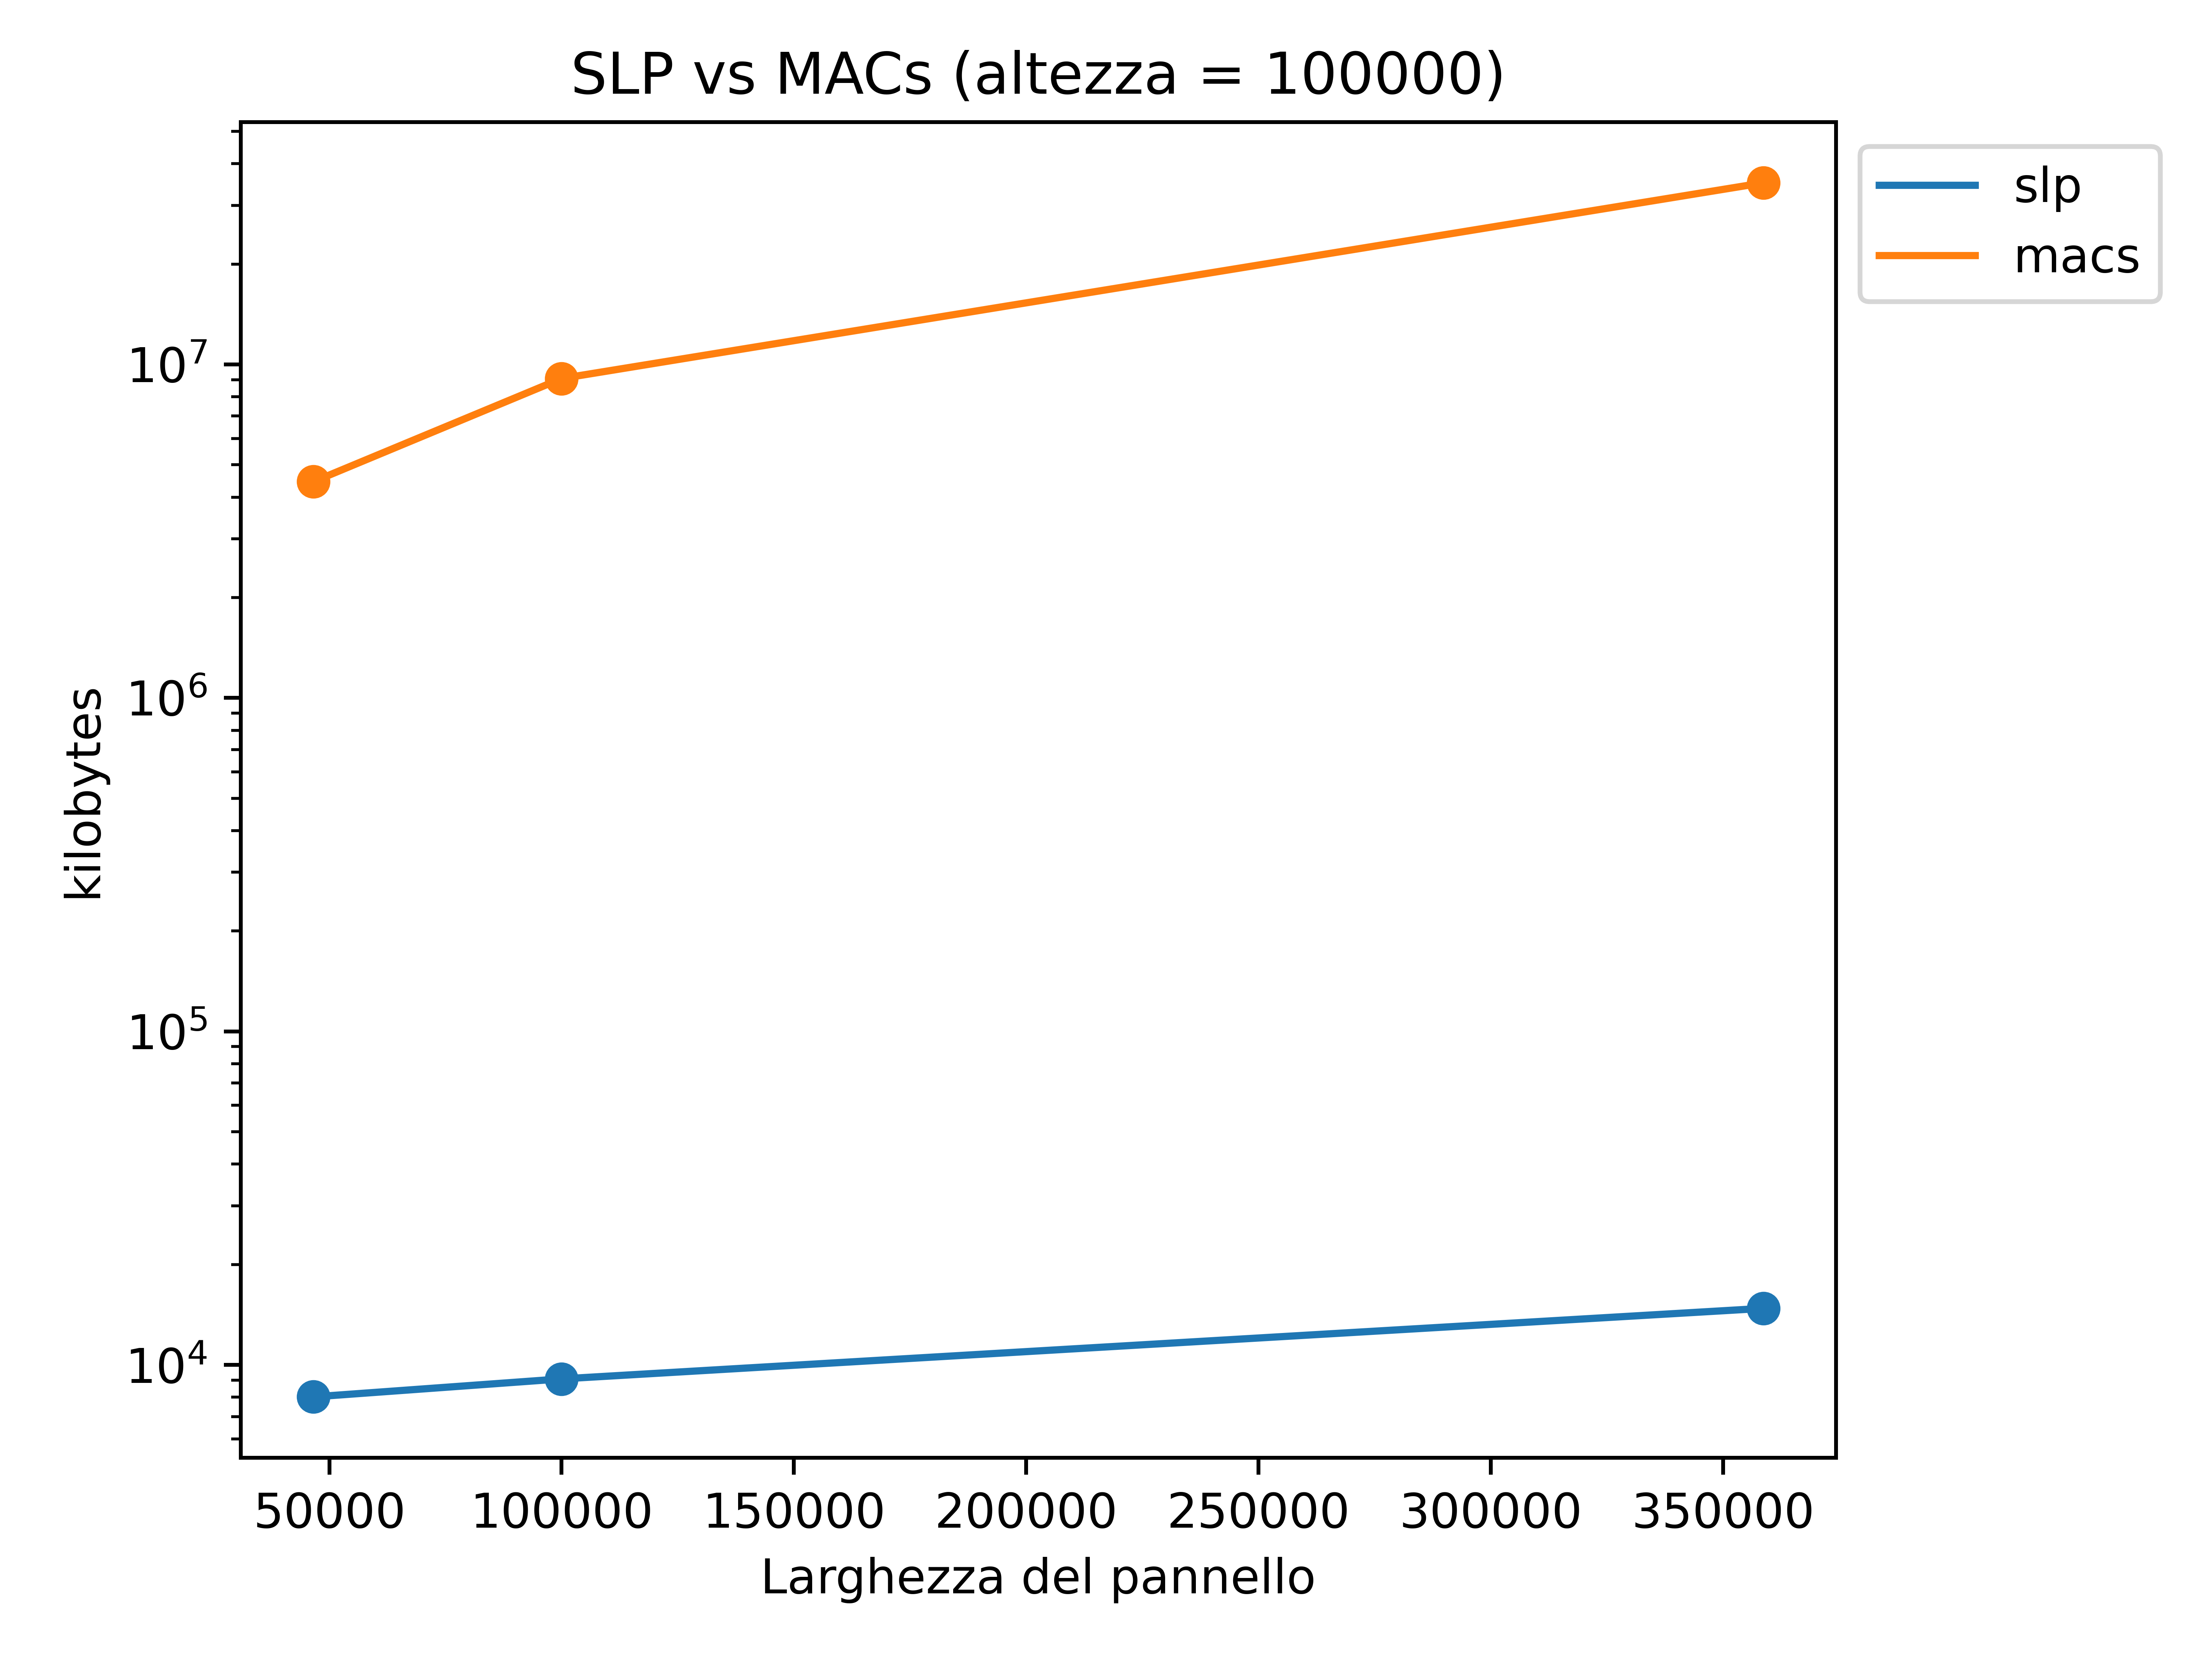
\includegraphics[scale = 0.6]{img/slp_vs_macs2.png}
  \caption{Confronto delle dimensioni, espresse in kilobytes, dei pannelli in
    formato \texttt{macs} e dei rispettivi \textit{SLP}. Il grafico è in scala
    logaritmica.}
  \label{fig:slpres2}
\end{figure}
Il caso estremo, un pannello $100000\times 358653$, occupante in memoria
circa 35gb in formato \texttt{.macs}, viene compresso in circa 15mb. Questo
accade soprattutto in quanto un pannello di soli simboli $\Sigma=\{0,1\}$
contiene molte ripetizioni, permettendo la costruzione di una grammatica,
tramite l'\textit{SLP}, particolarmente ``compatta''.
\subsubsection{Strutture dati}
Si analizzano ora le due strutture dati, confrontando lo spazio richiesto dalle
varie sotto-strutture per effettuare il match con una query esterna, descritte
alle sezioni \ref{secpbwt}, \ref{secrlpbwtnaive}, \ref{secrlpbwtbv} e
\ref{secrlpbwtms}.\\
Si precisa che i dati ora descritti sono stati calcolati nel seguente modo:
\begin{itemize}
  \item per quanto riguarda la \textbf{PBWT}, sfruttando le stime fatte da
  Durbin stesso
  \item per quanto riguarda la \textbf{RLPBWT}, sfruttando le serializzazioni
  ottenute tramite \textit{SDSL}
\end{itemize}
Con un studio al leggero variare del pannello si nota, graficamente in figura
\ref{memcomp1}, come quanto descritto precedentemente venga confermato. Le
informazioni richieste dall'algoritmo 5 di Durbin sono quelle che richiedono
maggior memoria mentre la variante della \textit{RLPBWT} basata su \textit{SLP}
e \textit{LCE query} risulta essere la soluzione migliore tra le varianti della
\textit{RLPBWT}. Bisogna però notare come la soluzione \textit{matchDynamic}
ritrovabile nella repository della \textit{PBWT} risulti essere incredibilmente
più efficace, avendo, secondo Durbin stesso, una richiesta in spazio
proporzionale a $\mathcal{O}(M+N)$. \\
Limitiamo però ora il confronto all'algoritmo 5 di Durbin, in quanto obbiettivo
della tesi. Da un punto di vista di guadagno percentuale in memoria i risultati
sembrano essere interessanti, confrontando tale soluzione con la migliore per la
\textit{RLPBWT}:
\begin{table}[H]
  \centering
  \footnotesize
  \begin{tabular}{c|c|c|c|c}
    \textbf{altezza} & \textbf{larghezza}
    & \textbf{RLPBWT SLP-LCE (\textit{kb})}
    & \textbf{PBWT Indexed (\textit{kb})} & \textbf{\%}\\
    \hline
    20000 & 4294 & 12118.62 & 1090270.65 & 1.1115\\
    21000 & 4294 & 12583.13 & 1144784.18 & 1.0992\\
    22000 & 4294 & 13033.78 & 1199297.71 & 1.0868\\
    23000 & 4294 & 13487.57 & 1253811.24 & 1.0757\\
    24000 & 4294 & 13954.44 & 1308324.78 & 1.0666\\
    25000 & 4294 & 14419.27 & 1362838.31 & 1.058\\
    26000 & 4294 & 14867.82 & 1417351.84 & 1.049\\
    27000 & 4294 & 15316.41 & 1471865.37 & 1.0406\\
    28000 & 4294 & 15765.41 & 1526378.9 & 1.0329\\
    29000 & 4294 & 16214.09 & 1580892.44 & 1.0256\\
  \end{tabular}
\end{table}
Provando in modo quantitativo l'efficacia in memoria della soluzione ultima
proposta in questa tesi.

% \begin{table}[H]
%   \centering
%   \tiny
%   \begin{tabular}{c|c|c|c|c|c|c|c|c}
%     \textbf{Altezza} & \textbf{Larghezza} & \textbf{Na\"{I}Ve}
%     & \textbf{Bitvector} & \textbf{Pannello}
%     & \textbf{SLP-Thr} & \textbf{SLP-LCE} & \textbf{Indexed}&
%                                                               \textbf{Dynamic}\\
%     \hline
%     20000 & 4294 & 116872.34 & 118842.8 & 22956.56 & 12422.86 & 12118.62
%                                                      & 1090270.65 & 20004.19\\
%     21000 & 4294 & 122717.92 & 124689.87 & 23954.83 & 12884.39 & 12583.13
%                                                        & 1144784.18 & 21004.19\\
%     22000 & 4294 & 128541.43 & 130509.84 & 24911.04 & 13337.4 & 13033.78
%                                                        & 1199297.71 & 22004.19\\
%     23000 & 4294 & 134383.15 & 136347.63 & 25900.01 & 13789.62 & 13487.57
%                                                        & 1253811.24 & 23004.19\\
%     24000 & 4294 & 140197.73 & 142157.96 & 26853.09 & 14239.5 & 13954.44
%                                                        & 1308324.78 & 24004.19\\
%     25000 & 4294 & 146047.34 & 148014.12 & 27855.43 & 14705.09 & 14419.27
%                                                        & 1362838.31 & 25004.19\\
%     26000 & 4294 & 151872.56 & 153834.89 & 28841.15 & 15154.06 & 14867.82
%                                                        & 1417351.84 & 26004.19\\
%     27000 & 4294 & 157711.32 & 159670.04 & 29793.47 & 15603.17 & 15316.41
%                                                        & 1471865.37 & 27004.19\\
%     28000 & 4294 & 163536.4 & 165489.58 & 30779.6 & 16052.56 & 15765.41
%                                                        & 1526378.9 & 28004.19\\
%     29000 & 4294 & 169381.28 & 171331.14 & 31765.37 & 16501.58 & 16214.09
%                                                        & 1580892.44 & 29004.19\\
    
%   \end{tabular}
% \end{table}
\begin{figure}
  \centering
  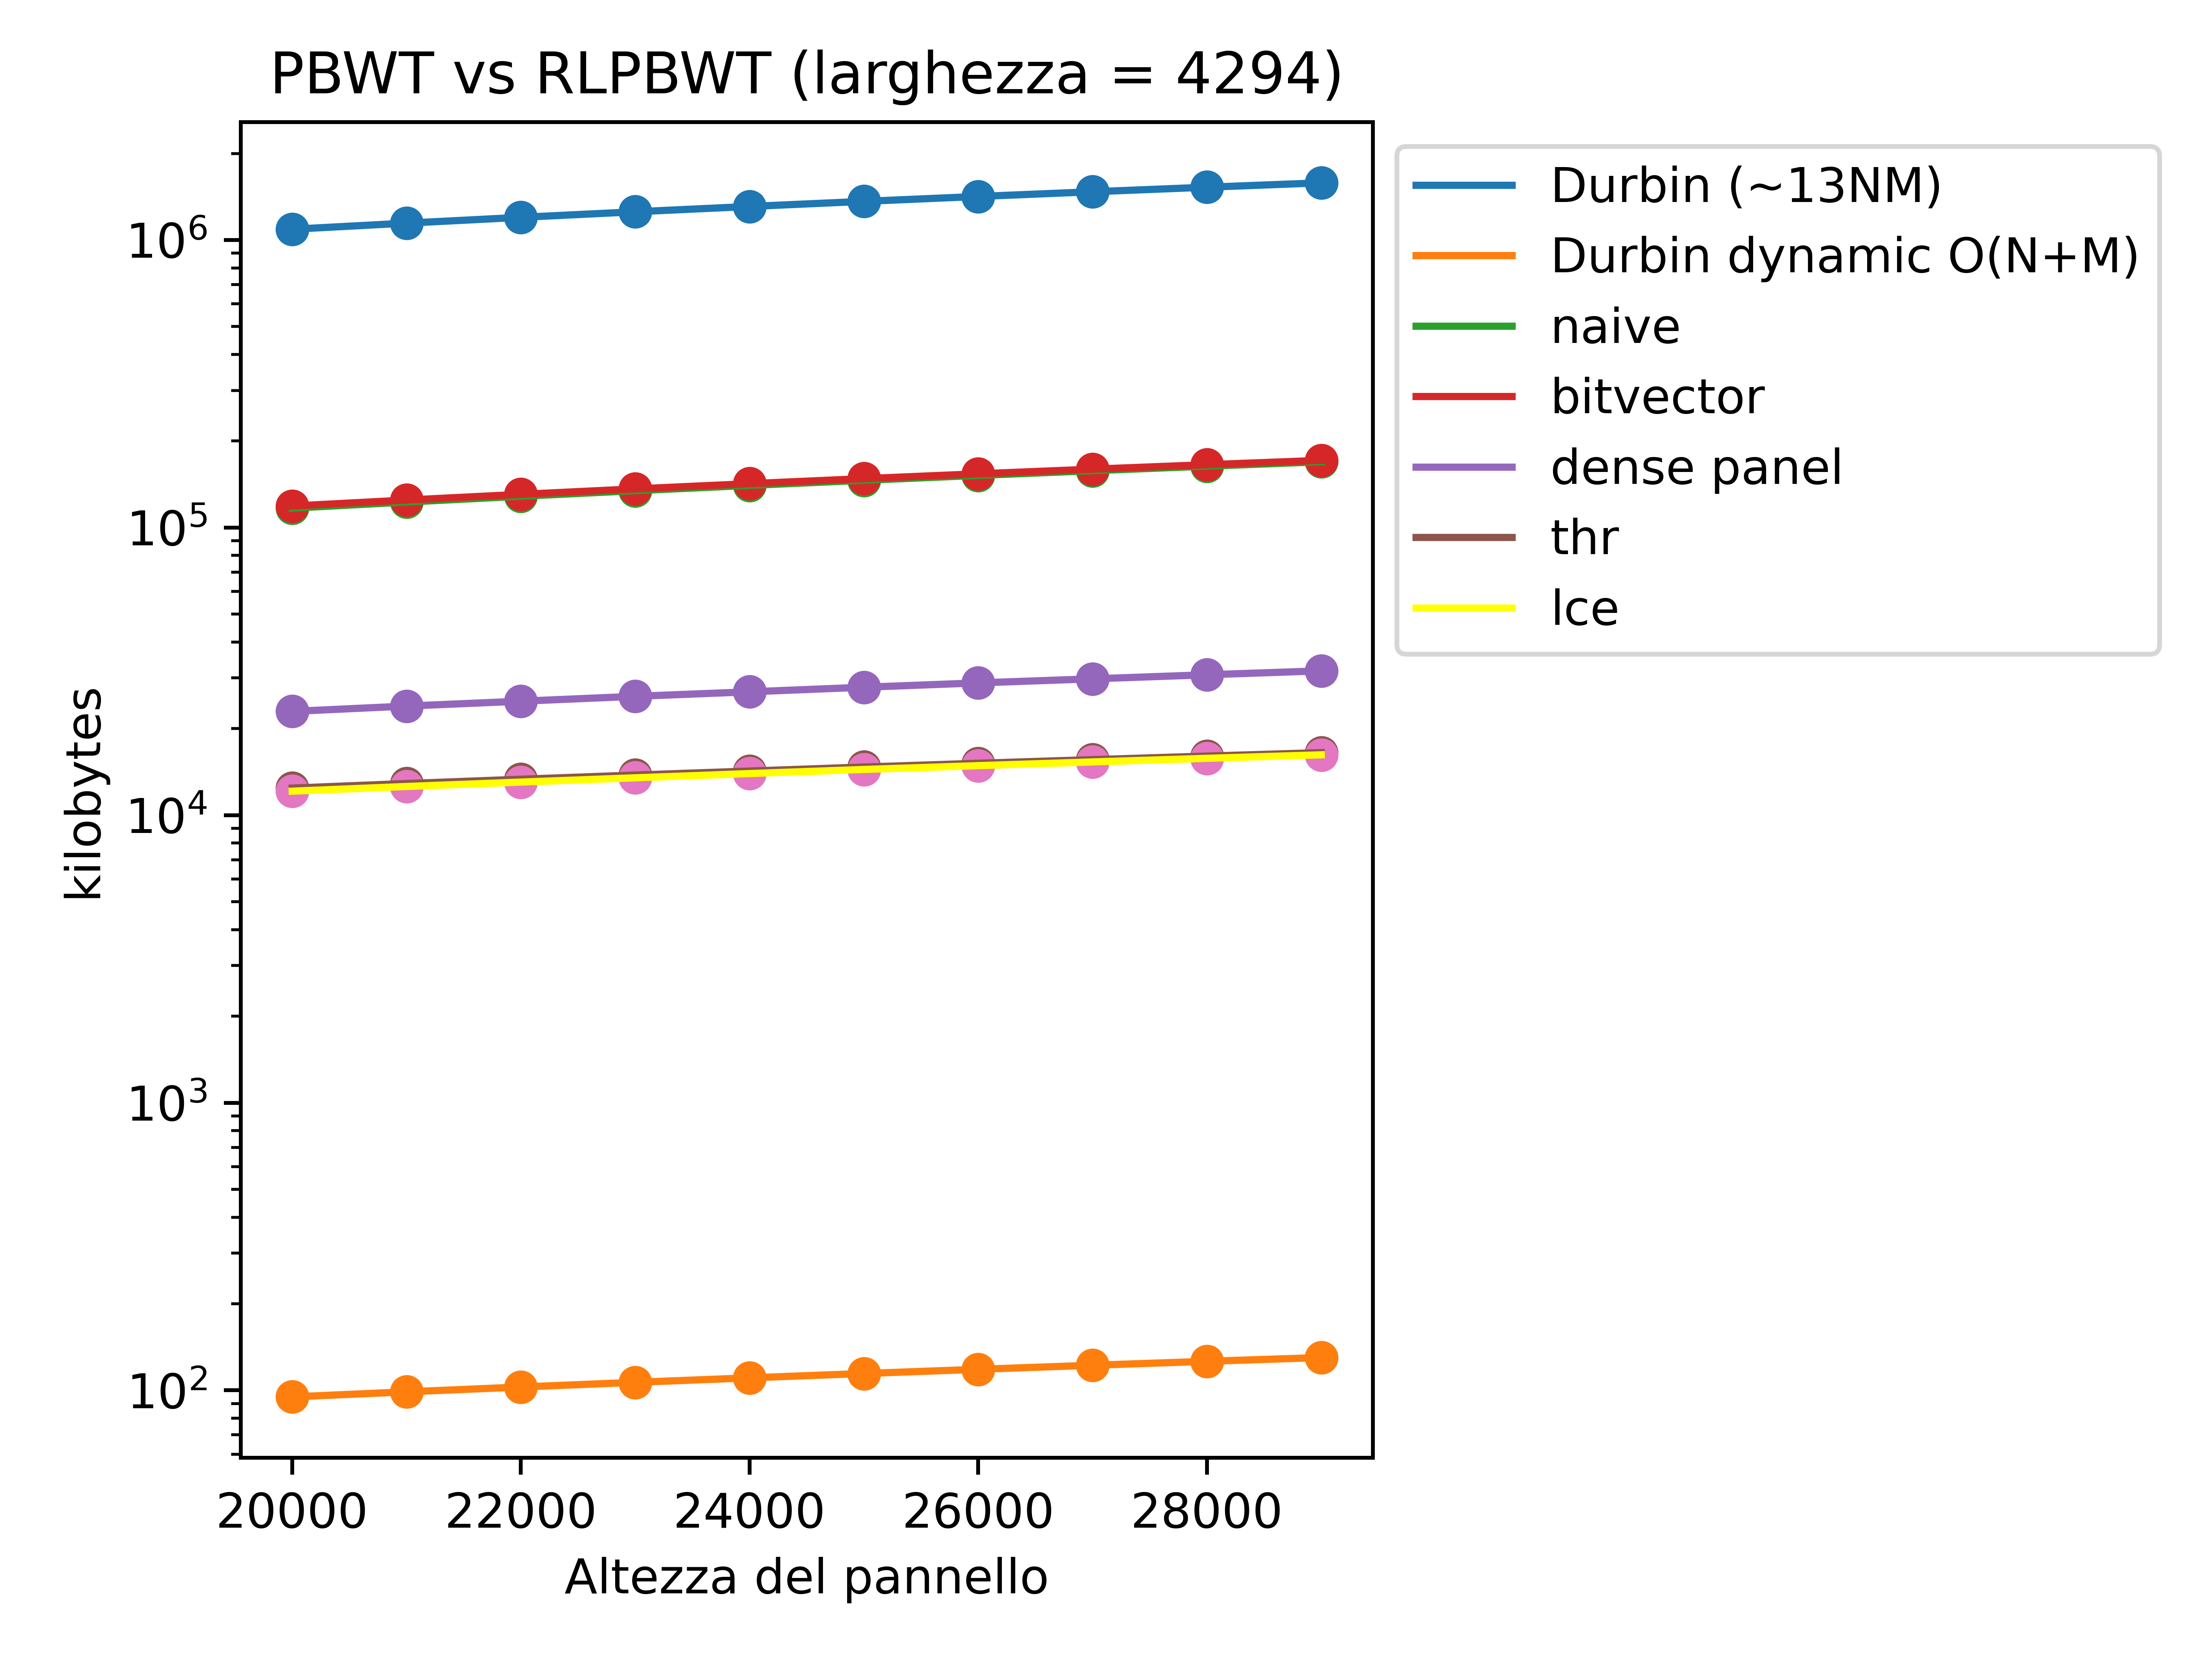
\includegraphics[scale = 0.6]{img/pbwt_vs_rlpbwt_dyn.png}
  \caption{Confronto dello spazio in memoria, in kilobytes, richiesto dalle
    varie strutture dati.} 
  \label{memcomp1}
\end{figure}
\subsection{Analisi temporale}
Bisogna infine considerare i tempi di esecuzione per il pattern matching con un
pannello di query. Dal punto di vista della \textit{RLPBWT} bisogna considerare
in primis due aspetti:
\begin{itemize}
  \item avere meno informazione in memoria comporta molto probabilmente, a
  parità di risultati, tempi maggiori
  \item l'uso di strutture dati succinte ed eventualmente dell'\textit{SLP}
  comporta costi dal punto di vista temporale. Come anticipato in sezione
  \ref{bvsec}, le operazioni sugli sparse bitvector non sono tutte i tempo
  costante e, come invece anticipato in sezione \ref{slpsec}, gli \textit{SLP}
  non garantiscono \textit{random access} in tempo costante e questo, per quanto
  poi l'algoritmo di estensione sia efficiente, si ripercuote anche sul calcolo
  delle \textit{LCE query}
\end{itemize}
Questa premessa fa capire come ci si aspettasse che i tempi fossero maggiori con
la \textit{RLPBWT}, in ogni sua variante, rispetto all'algoritmo 5 di Durbin.
Parlando invece dell'algoritmo \textit{matchDynamic} si ha che, per quanto
asintoticamente presenti la stessa complessità dell'algoritmo 5, ovvero
$\mathcal{O}(N(M+Q))$, con $Q$ numero di query, esso risulta incredibilmente più
performante. \\
Alcuni risultati sono visualizzabili in figura \ref{fig:1000} e \ref{fig:10000},
dove si possono osservare sia i tempi che lo spazio richiesto. Anche la completa
esecuzione quindi conferma come l'algoritmo 5 sia incredibilmente esoso dal
punto di vista dello spazio richiesto, pur avendo ottime performance
temporali. Dal punto di vista invece delle varianti della \textit{RLPBWT} si
nota come:
\begin{itemize}
  \item la \textit{RLPBWT na\"{i}ve}, priva dell'uso dei bitvector e
  dell'\textit{SLP}, risulti essere la più performante, anche se, si ricordi,
  non permette di identificare quali righe stiano effettivamente matchando ma
  solo quante
  \item la \textit{RLPBWT con bitvector}, avente lo stesso limite della variante
  na\"{i}ve, presenta anche maggiori costi in termini di memoria di quest'ultima,
  avendo anch'essa ancora l'\textit{LCP array} completo ma anche tutte le
  informazioni memorizzate in bitvector, che aumentano, come anticipato, i tempi
  di calcolo. La chiave delle varianti che sfruttano
  le \textit{matching statistics} è infatti quella di non avere l'\textit{array
    LCP} in memoria, una delle cause principali dell'aumento di spazio richiesto
  \item le tre varianti basate sulle \textit{matching statistics} hanno spazio
  occupato pressoché uguale, anche se si può percepire, nei due casi studiati,
  come il tenere l'intero pannello in forma di bitvector, all'aumentare della
  grandezza dello stesso, comporti molta più memoria degli \textit{SLP}. Dal
  punto di vista temporale, inoltre, anche se si ha \textit{random access} in
  tempo costante, all'aumentare del pannello, il numero di accessi allo stesso
  comporta forti costi in termini di tempo macchina. Questi
  ultimi, infatti, come già visto occupano pochissima memoria anche con pannelli
  molto estesi. Dal punto di vista temporale si rileva come la variante basata
  su \textit{SLP} e \textit{threshold} richieda molto più tempo. Si nota che ciò
  accade a causa di due fattori:
  \begin{itemize}
    \item il continuo accesso all'\textit{SLP} per calcolare $MS[i].len$
    \item l'eventuale accesso all'\textit{SLP} per disambiguare le threshold a
    fine run
  \end{itemize}
  Tra le tre quindi la variante con \textit{SLP} e \textit{LCE query},
  all'aumentare della grandezza del pannello, risulta essere la soluzione
  migliore
\end{itemize}

\begin{figure}
  \centering
  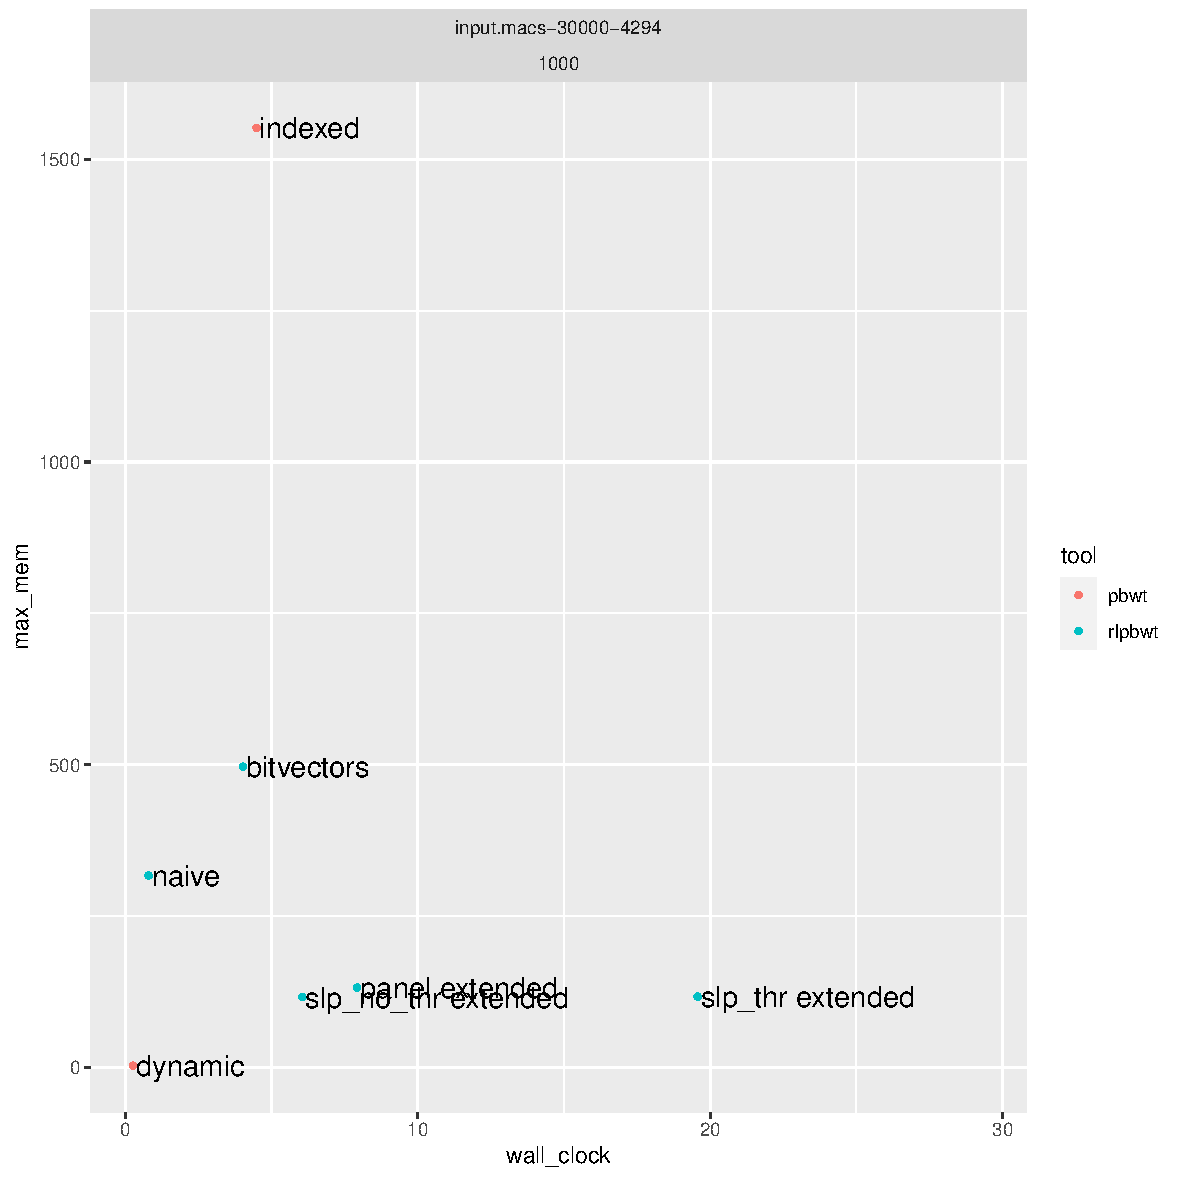
\includegraphics[scale = 0.35]{img/time_vs_mem_1000.pdf}
  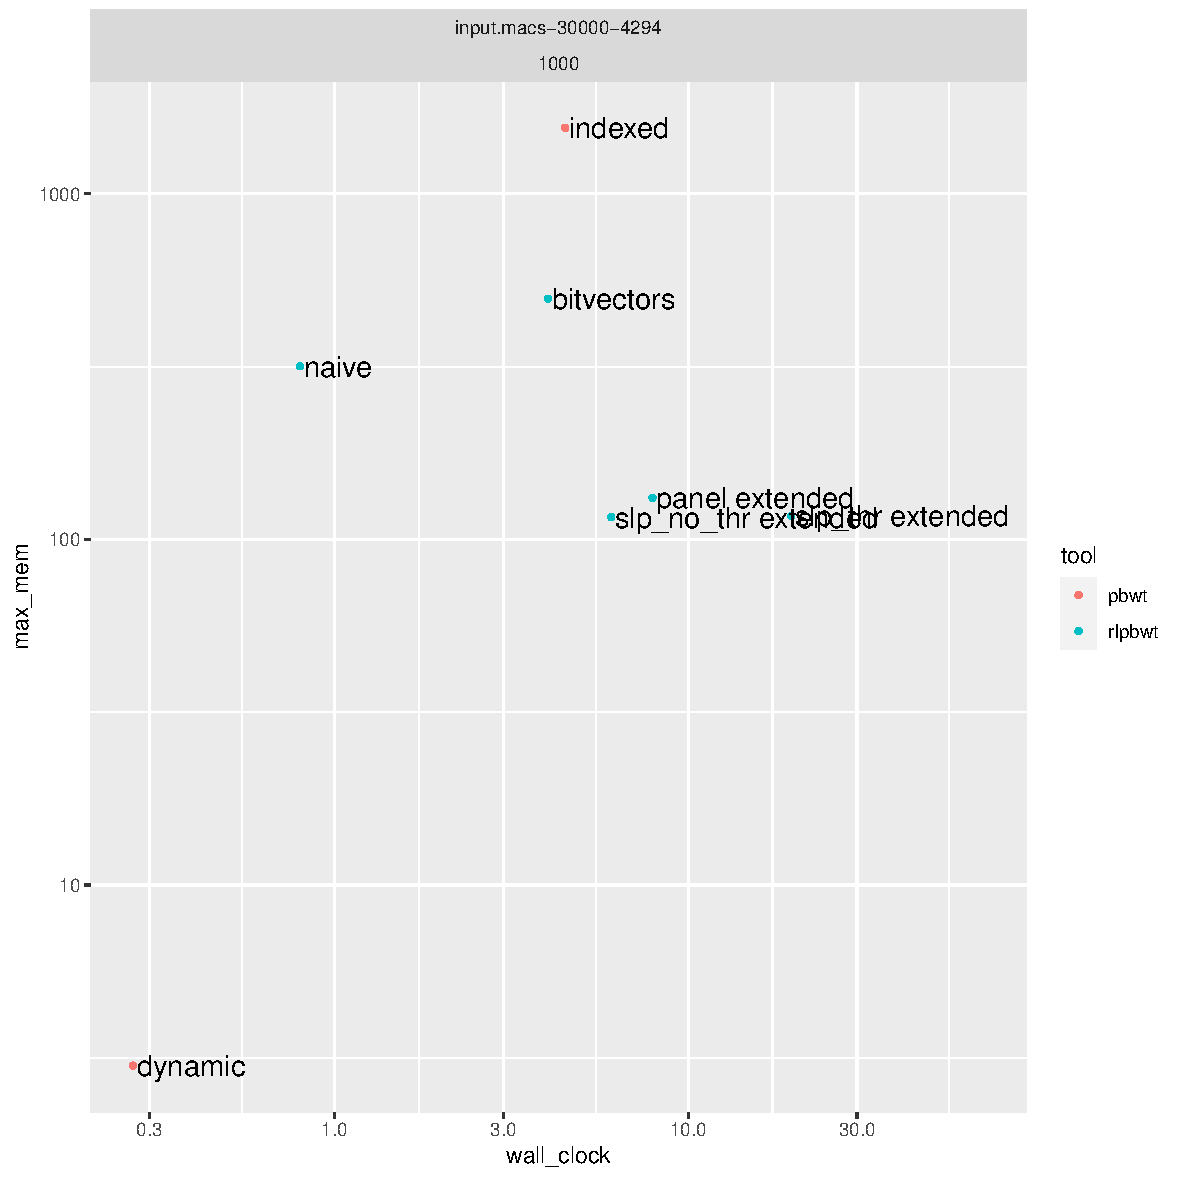
\includegraphics[scale = 0.35]{img/time_vs_mem-loglog_1000.pdf}
  \caption{Esecuzione dei vari algoritmi di match su un pannello
    $29000\times 4294$ e 1000 query.  Il grafico a destra è in scala
    logaritmica. }
  \label{fig:1000}
\end{figure}

\begin{figure}
  \centering
  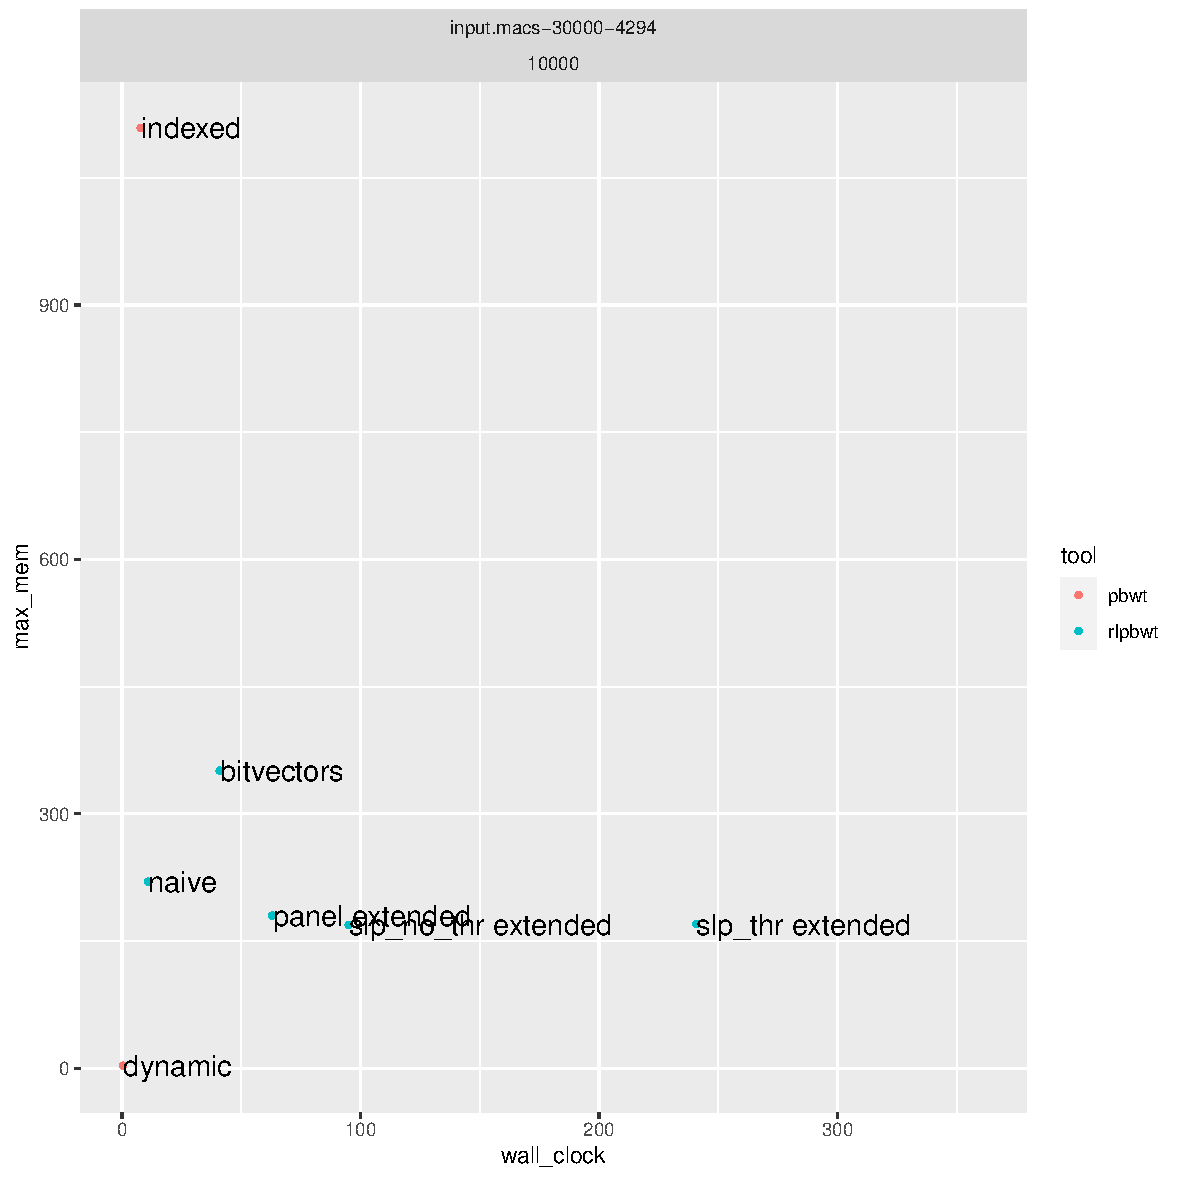
\includegraphics[scale = 0.35]{img/time_vs_mem_10000.pdf}
  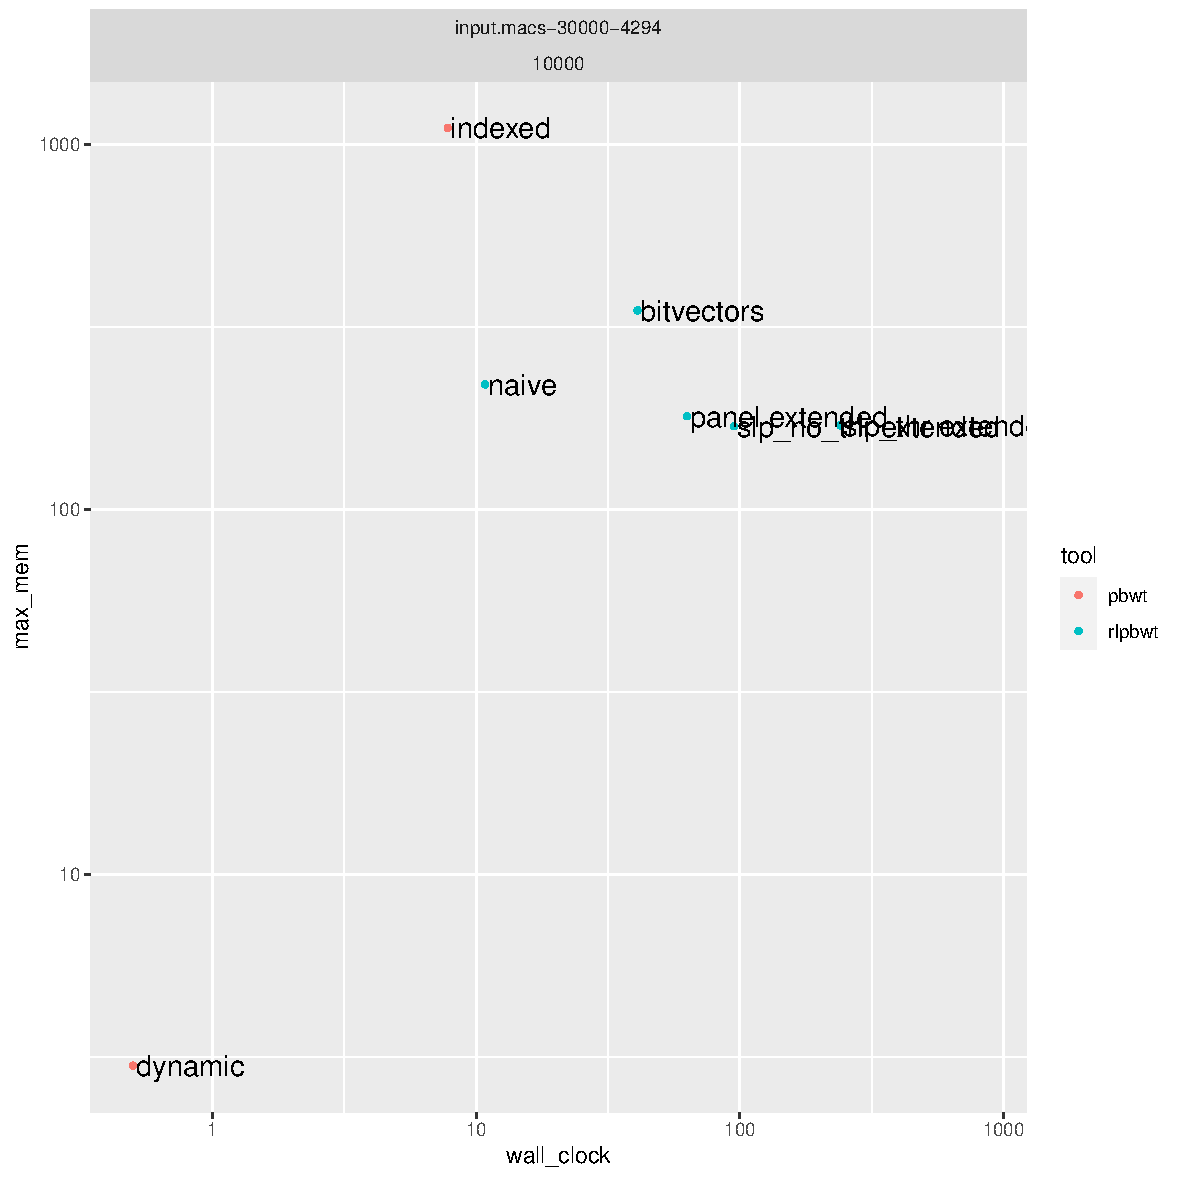
\includegraphics[scale = 0.35]{img/time_vs_mem-loglog_10000.pdf}
  \caption{Esecuzione dei vari algoritmi di match su un pannello
    $20000\times 4294$ e 10000 query. Il grafico a destra è in scala
    logaritmica. }
  \label{fig:10000}
\end{figure}
Per completezza, in figura \ref{fig:bigres}, si riportano anche i risultati in
tempo 
e spazio di una sperimentazione su un pannello di grandi dimensioni:
$70000\times 46538$ con $30000$ query. Sono riportati anche i risultati delle
tre varianti basate su \textit{matching statistics} senza l'estensione dei match
tramite le \textbf{funzioni} $\boldsymbol \varphi$ e
$\boldsymbol\varphi^{\mathbf{-1}}$. Si può notare come la struttura dati aggiuntiva
non comporti praticamente alcuna differenza sostanziale sia in termini di
memoria che di tempo di calcolo. In merito agli altri risultati si ha che
seguono tutti il trend già descritto negli esempi precedenti. In particolare si
nota che:
\begin{itemize}
  \item l'algoritmo 5 di Durbin ha una richiesta di memoria davvero molto
  grande, parlando di circa 40.75 gb di memoria richiesta
  \item l'algoritmo \textit{matchDynamic} di Durbin risulta essere migliore sia
  dal punto di vista dello spazio richiesto che del tempo d'esecuzione. Parlando
  di tempi, infatti, l'intera esecuzione richiede $\sim 22$s, contro i $\sim
  411$ dell'algoritmo \textit{matchIndexed} e i $\sim 1824$ della
  \textit{RLPBWT} con \textit{SLP} e \textit{LCE query}
  \item la variante \textit{RLPBWT} con \textit{SLP} e \textit{threshold}, per
  le problematiche già descritte richiede un tempo d'esecuzione importante,
  parlando di circa 2 ore di esecuzione
\end{itemize}
\begin{figure}
  \centering
  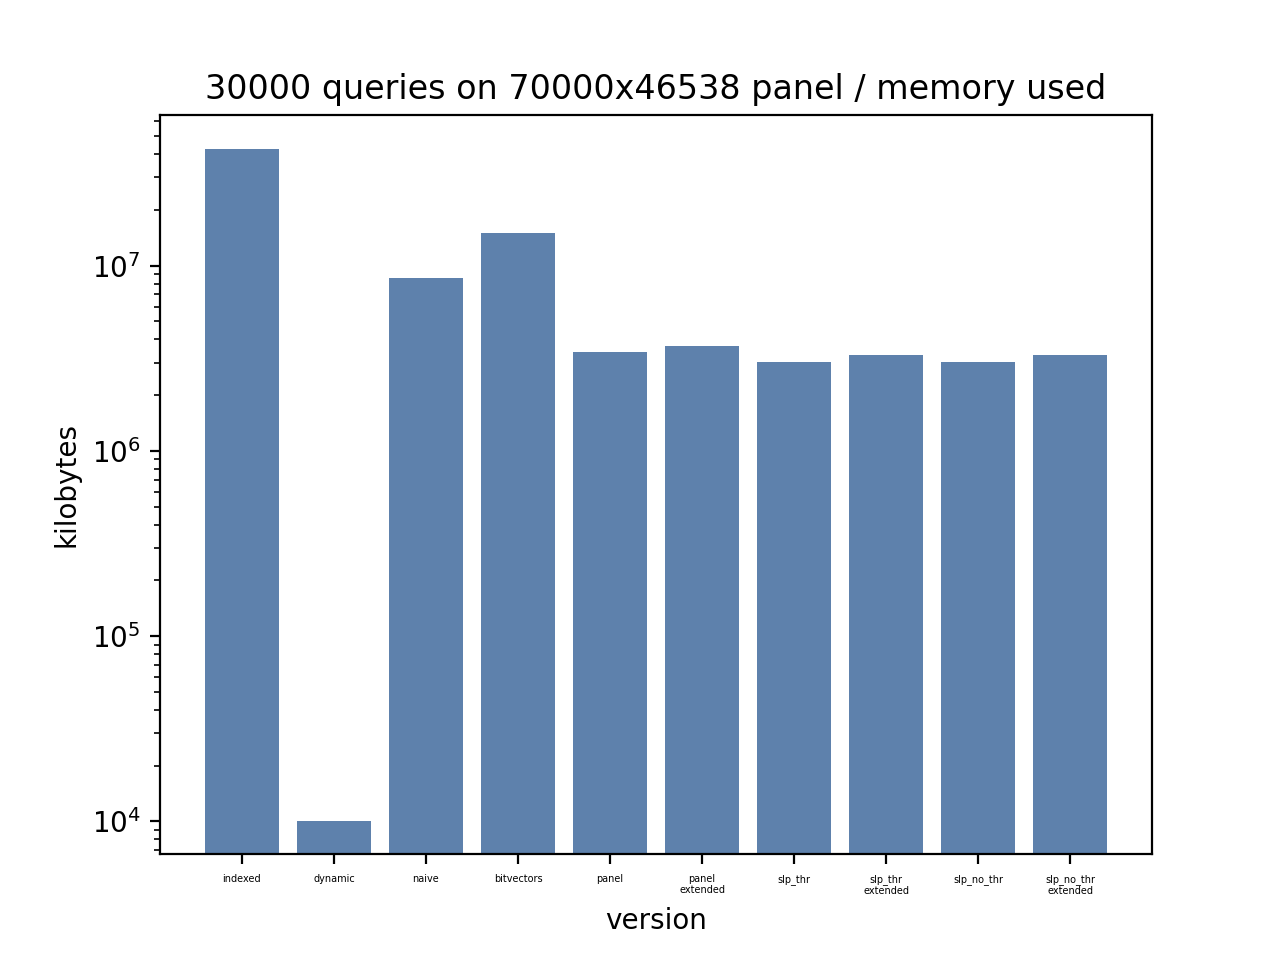
\includegraphics[scale = 0.4]{img/mem.png}
  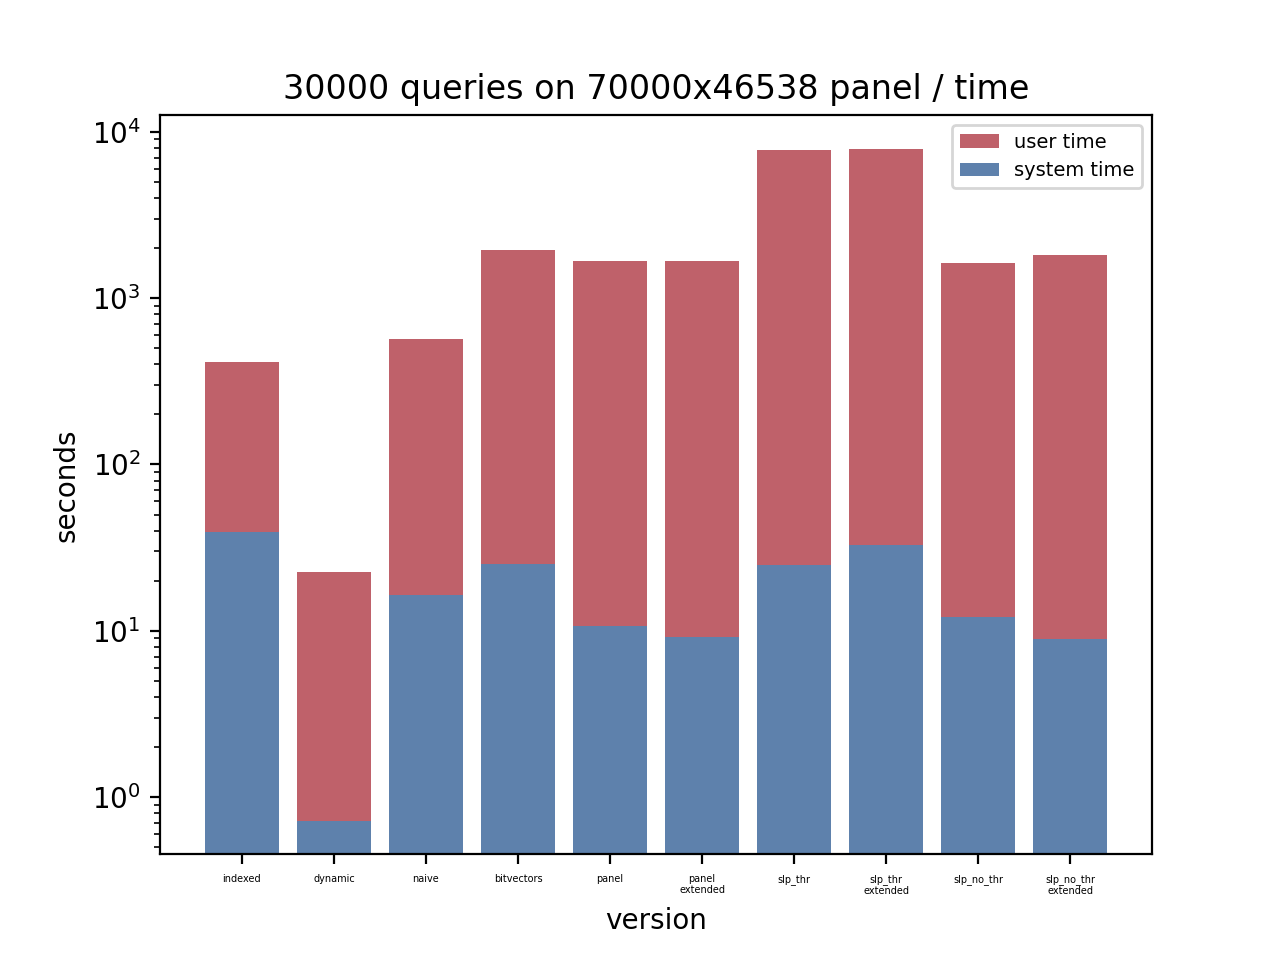
\includegraphics[scale = 0.4]{img/time.png}
  \caption{Risultati, in scala logaritmica, dell'esecuzione dei vari algoritmi
    su un pannello di grosse dimensioni. Si noti che, quantitativamente, la
    variante \textit{matchIndexed} richieda $42736132$ kb di memoria mentre la
    \textit{RLPBWT} con \textit{SLP} e \textit{LCE query} solo $3286424$ kb,
    richiedendo quindi appena il 7\% di memoria richiesta dall'algoritmo 5 di
    Durbin. Infine, per quanto la scala logaritmica renda impercettibile tale
    differenza, la variante \textit{RLPBWT} con pannello richiede $3695968$ kb,
    quindi circa $380$ mb in più della soluzione basata sull'uso
    dell'\textit{SLP}. } 
  \label{fig:bigres}
\end{figure}

